\section{How Does Convolution Work?}
\begin{frame}{}
    \LARGE CNN: \textbf{How Does Convolution Work?}
\end{frame}

\begin{frame}[allowframebreaks]{How Does Convolution Work?}

\begin{figure}
\centering
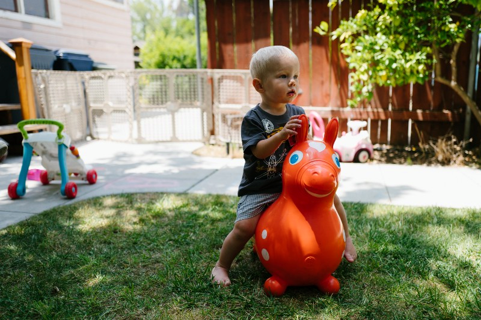
\includegraphics[width=1.0\textwidth,height=0.8\textheight,keepaspectratio]{images/cnn/conv_2.png}
\caption*{\scriptsize [Source: \url{https://www.flickr.com/photos/99146227@N00/}]}
\end{figure}

\framebreak

\begin{figure}
\centering
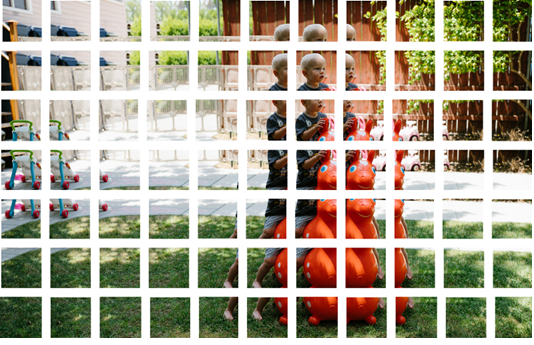
\includegraphics[width=1.0\textwidth,height=0.8\textheight,keepaspectratio]{images/cnn/conv_3.png}
\caption*{\scriptsize [Source: \url{https://medium.com/the-mission/up-to-speed-on-deep-learning-july-update-part-2-baacc835d8ab}]}
\end{figure}

\framebreak

\begin{figure}
\centering
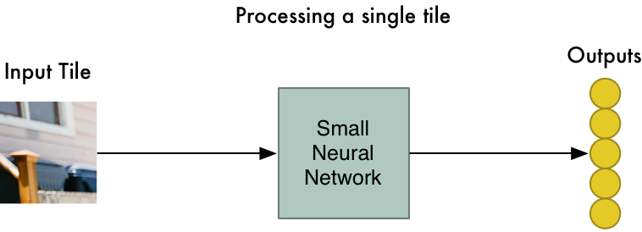
\includegraphics[width=1.0\textwidth,height=0.8\textheight,keepaspectratio]{images/cnn/conv_4.png}
\caption*{\scriptsize [Source: \url{https://www.researchgate.net/figure/An-input-tile-processed-through-neural-network_fig5_333507222}]}
\end{figure}

\framebreak

\begin{figure}
\centering
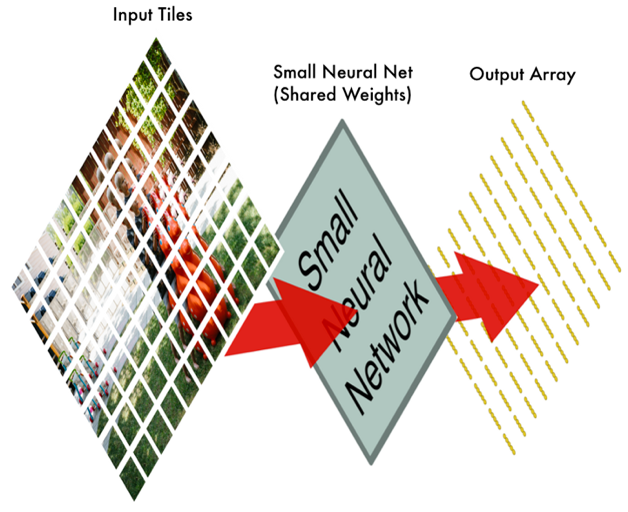
\includegraphics[width=1.0\textwidth,height=0.8\textheight,keepaspectratio]{images/cnn/conv_5.png}
\caption*{\scriptsize [Source: \url{https://medium.com/@ageitgey/machine-learning-is-fun-part-3-deep-learning-and-convolutional-neural-networks-f40359318721}]}
\end{figure}

\framebreak

\begin{figure}
\centering
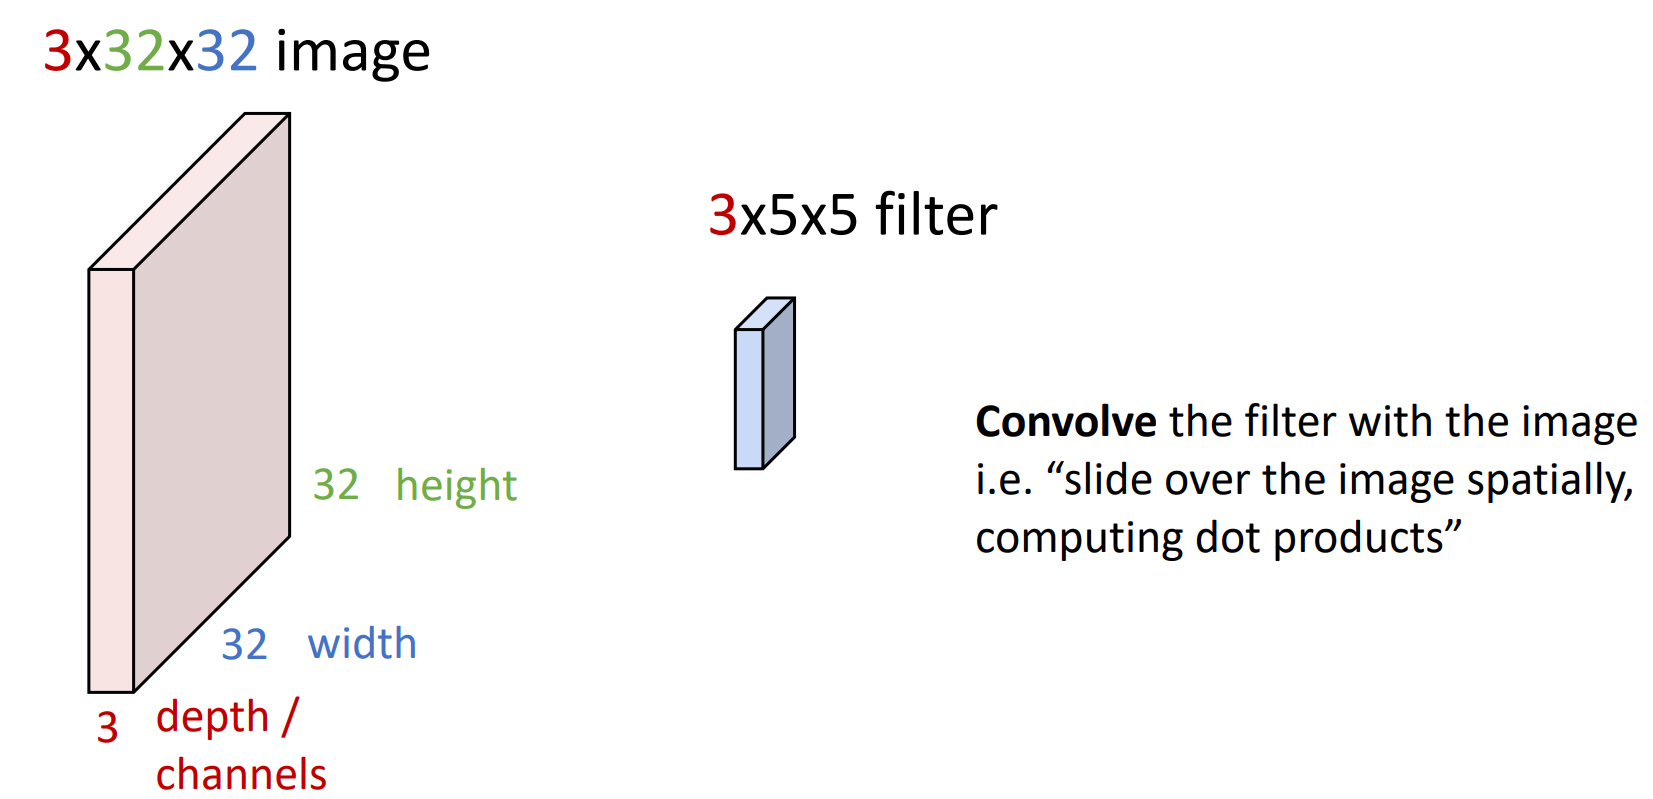
\includegraphics[width=1.0\textwidth,height=0.8\textheight,keepaspectratio]{images/cnn/conv_6.png}
\caption*{\scriptsize [Source: \url{https://cs229.stanford.edu/notes2022fall/cs229-conv_nets_slides.pdf}]}
\end{figure}

\framebreak

\begin{figure}
\centering
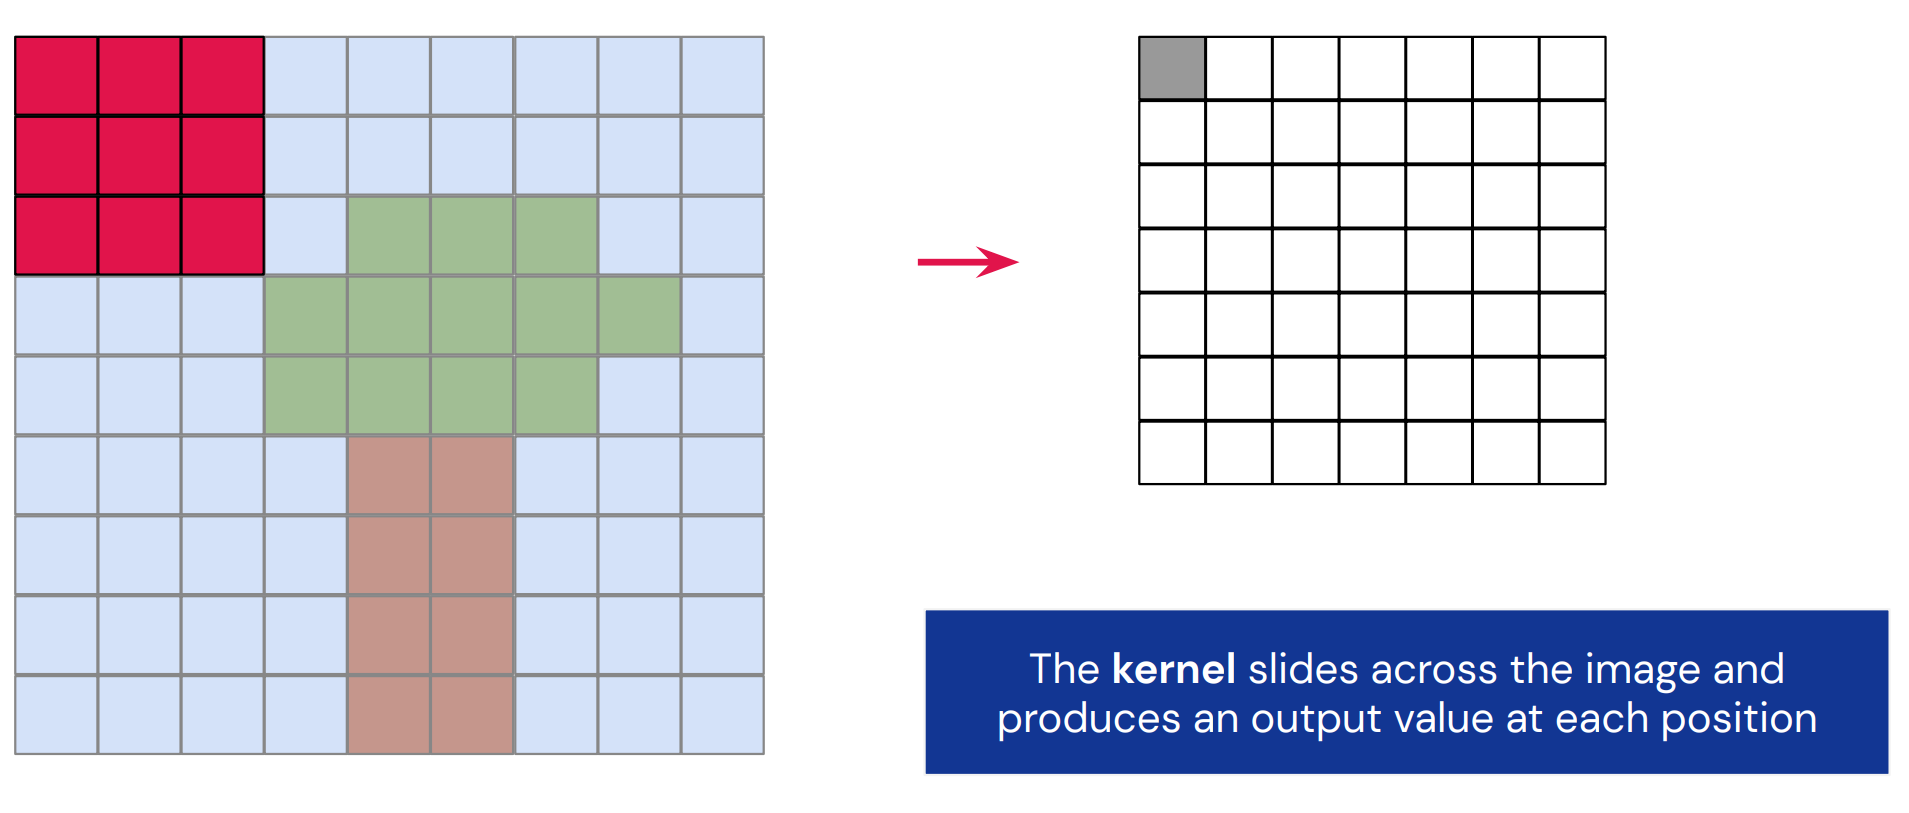
\includegraphics[width=1.0\textwidth,height=0.8\textheight,keepaspectratio]{images/cnn/conv_7.png}
\caption*{\scriptsize [Source: \url{https://medium.com/@mohamedhedifkir/convolutional-neural-network-23a6acb08d6a}]}
\end{figure}

\framebreak

\begin{figure}
\centering
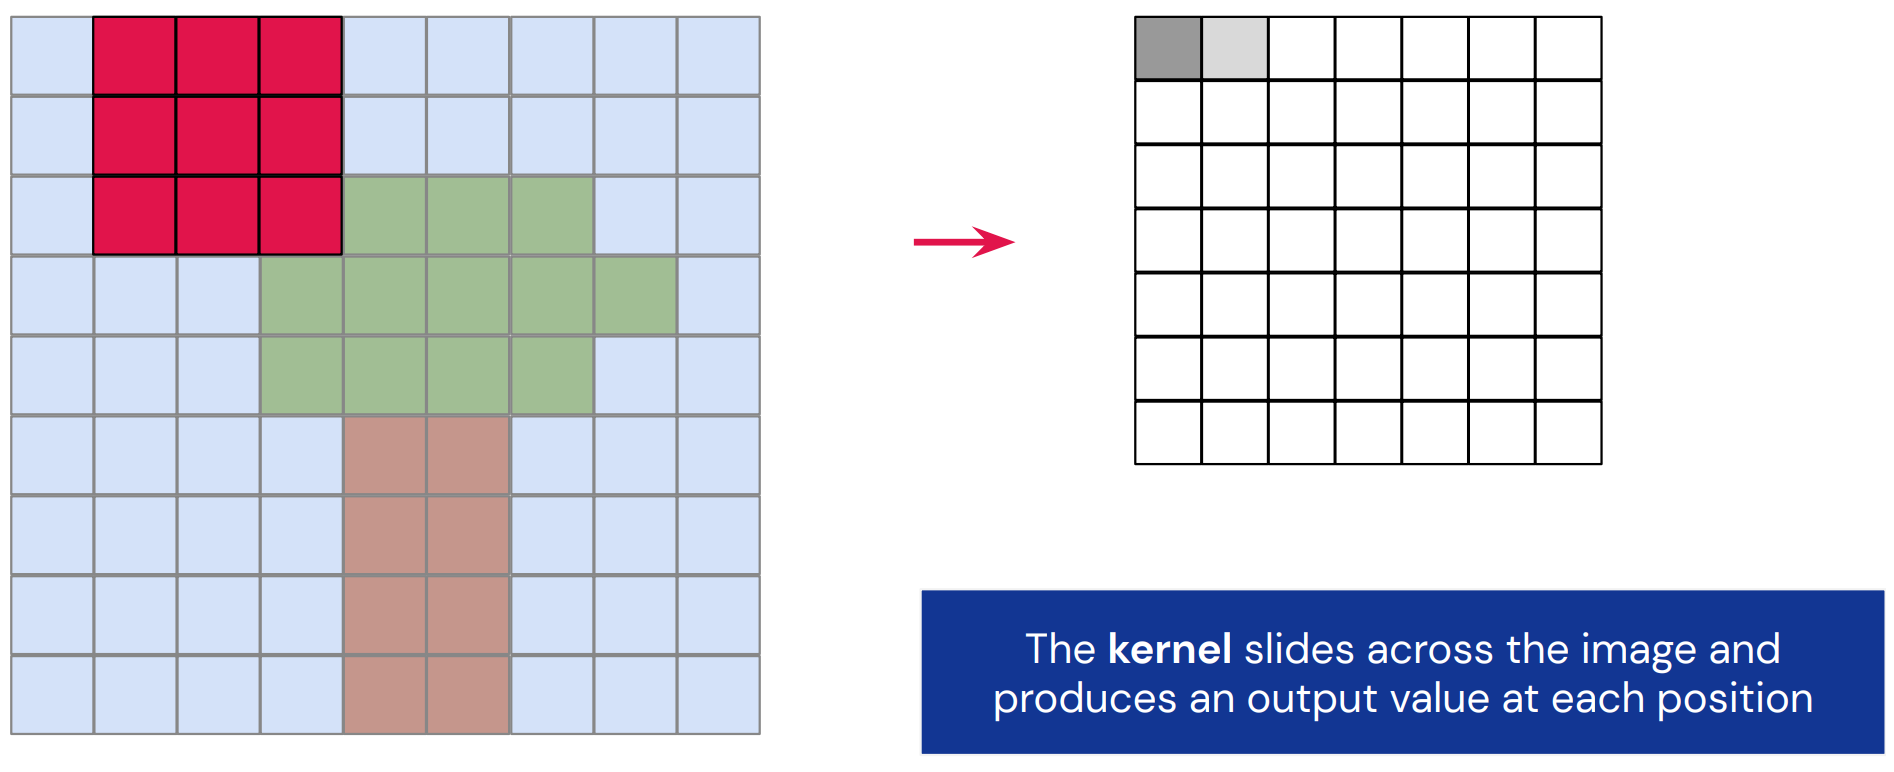
\includegraphics[width=1.0\textwidth,height=0.8\textheight,keepaspectratio]{images/cnn/conv_8.png}
\caption*{\scriptsize [Source: \url{https://medium.com/@mohamedhedifkir/convolutional-neural-network-23a6acb08d6a}]}
\end{figure}

\framebreak

\begin{figure}
\centering
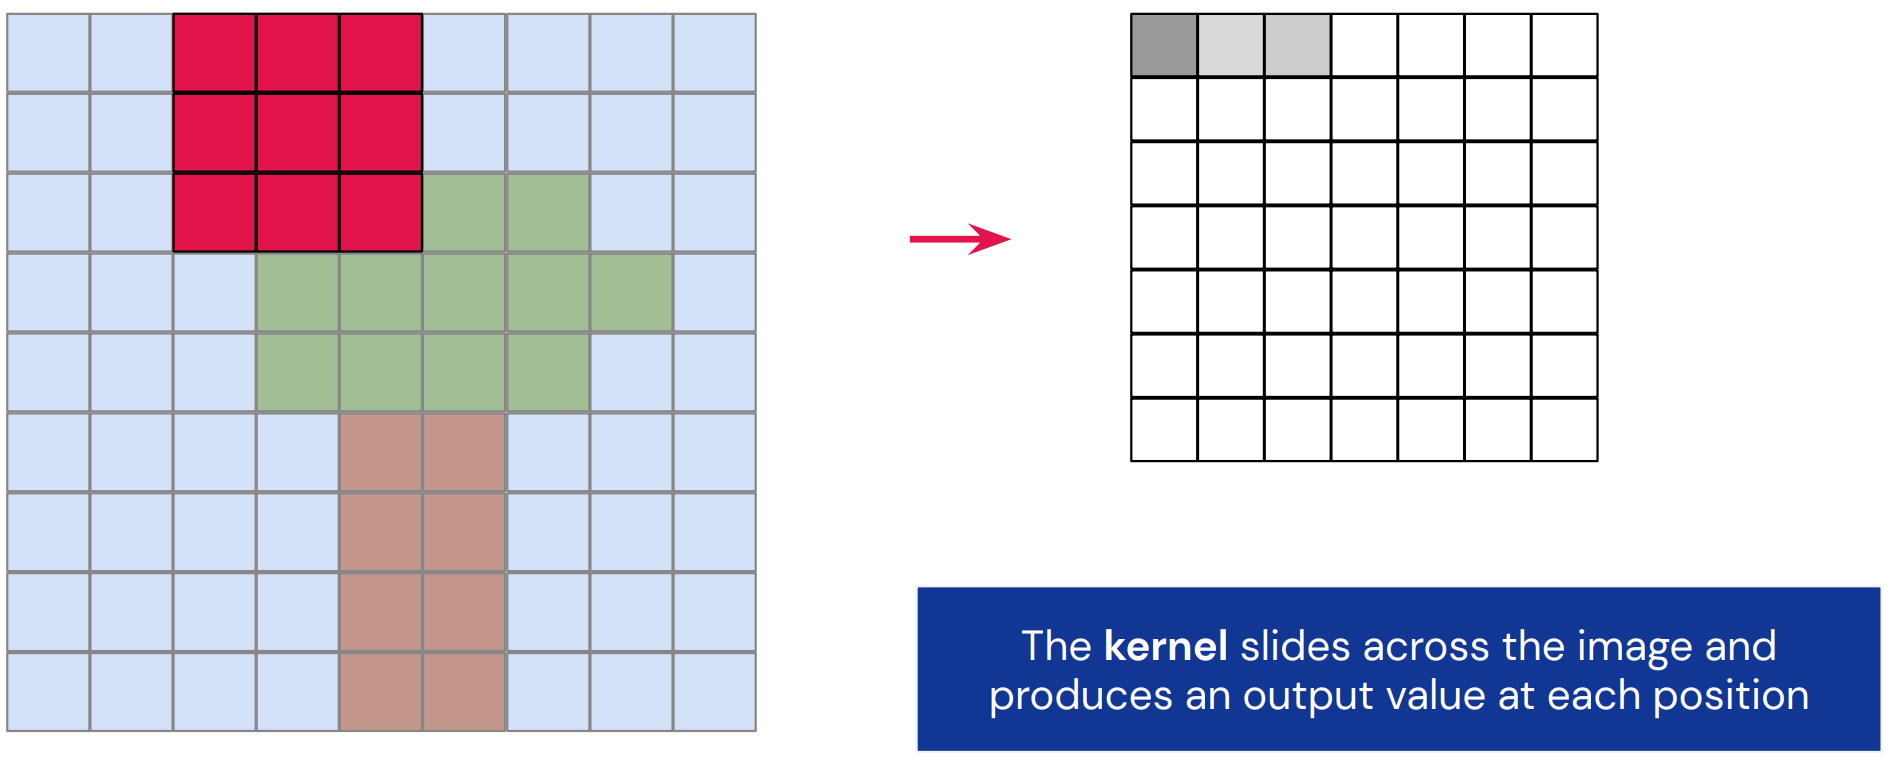
\includegraphics[width=1.0\textwidth,height=0.8\textheight,keepaspectratio]{images/cnn/conv_9.png}
\caption*{\scriptsize [Source: \url{https://medium.com/@mohamedhedifkir/convolutional-neural-network-23a6acb08d6a}]}
\end{figure}

\framebreak

\begin{figure}
\centering
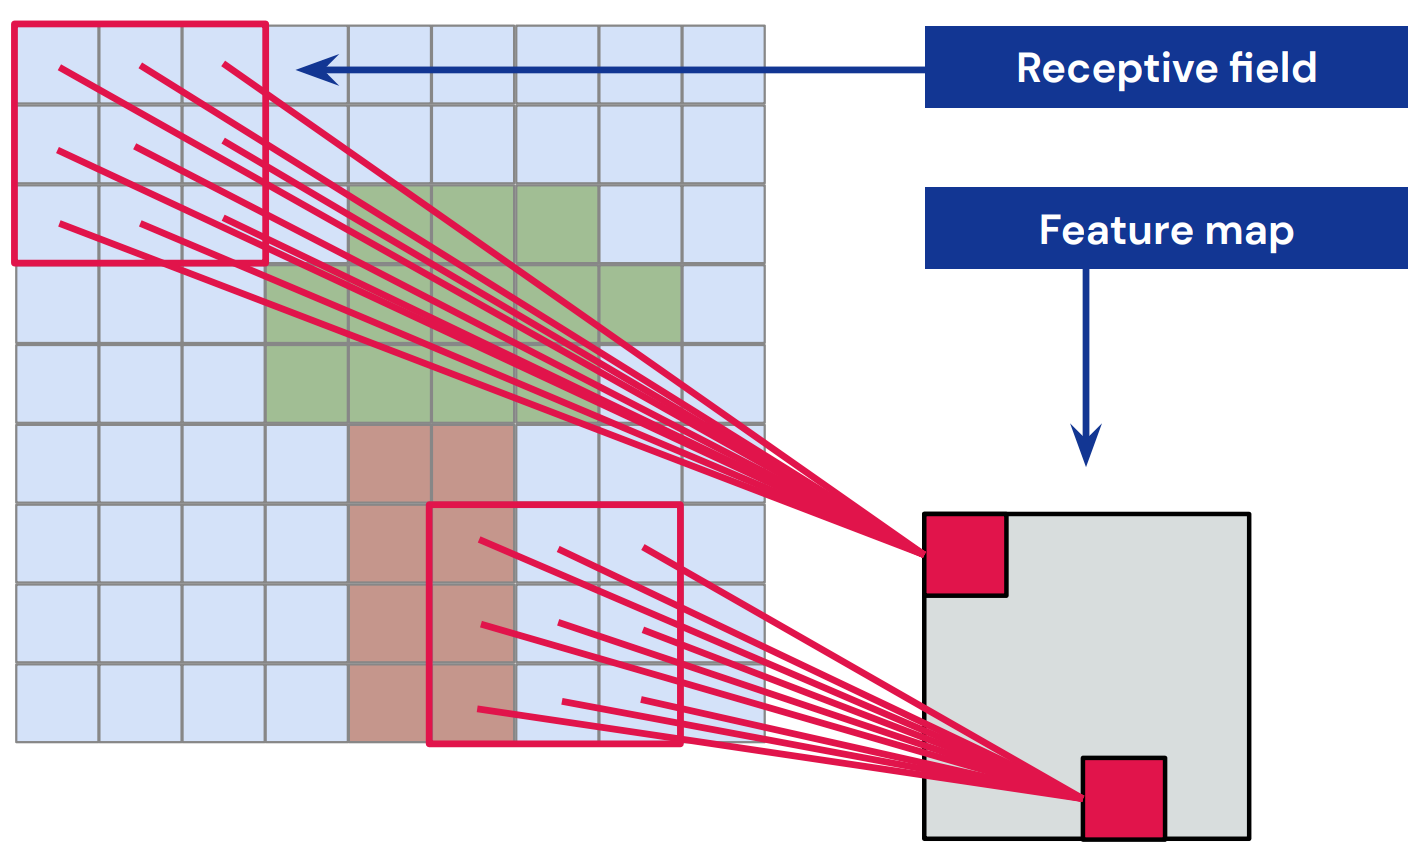
\includegraphics[width=1.0\textwidth,height=0.8\textheight,keepaspectratio]{images/cnn/conv_10.png}
\caption*{\scriptsize [Source: \url{https://medium.com/@nghihuynh_37300/convolutional-neural-networks-for-image-recognition-7148a19f981f}]}
\end{figure}

\framebreak

\begin{figure}
\centering
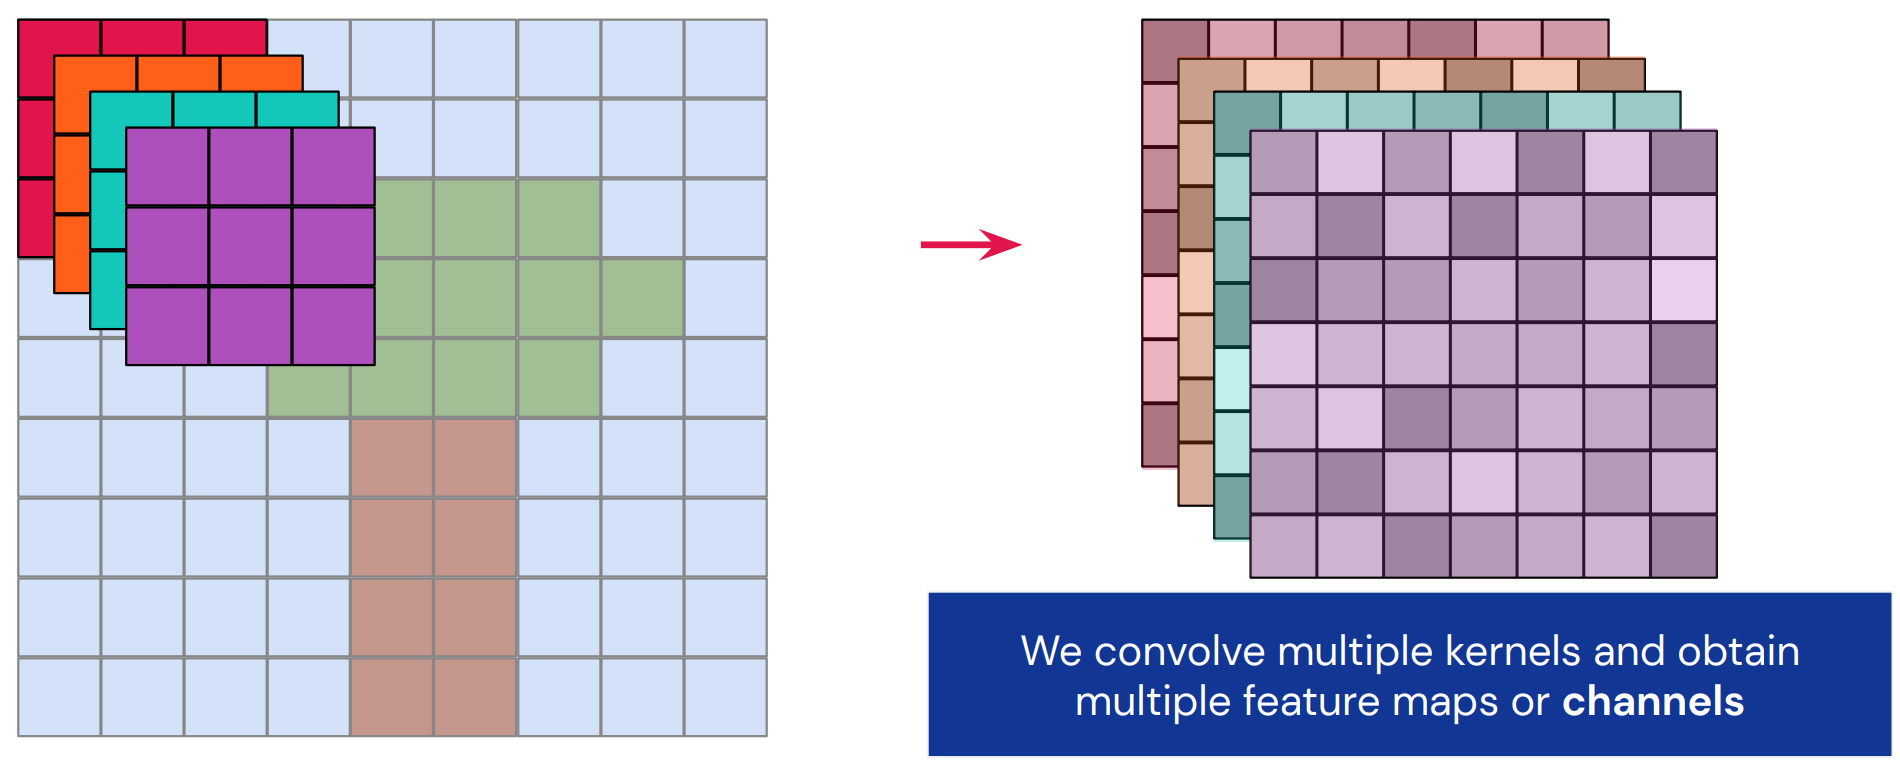
\includegraphics[width=1.0\textwidth,height=0.8\textheight,keepaspectratio]{images/cnn/conv_11.png}
\caption*{\scriptsize [Source: \url{https://medium.com/@nghihuynh_37300/convolutional-neural-networks-for-image-recognition-7148a19f981f}]}
\end{figure}

\framebreak

\begin{figure}
\centering
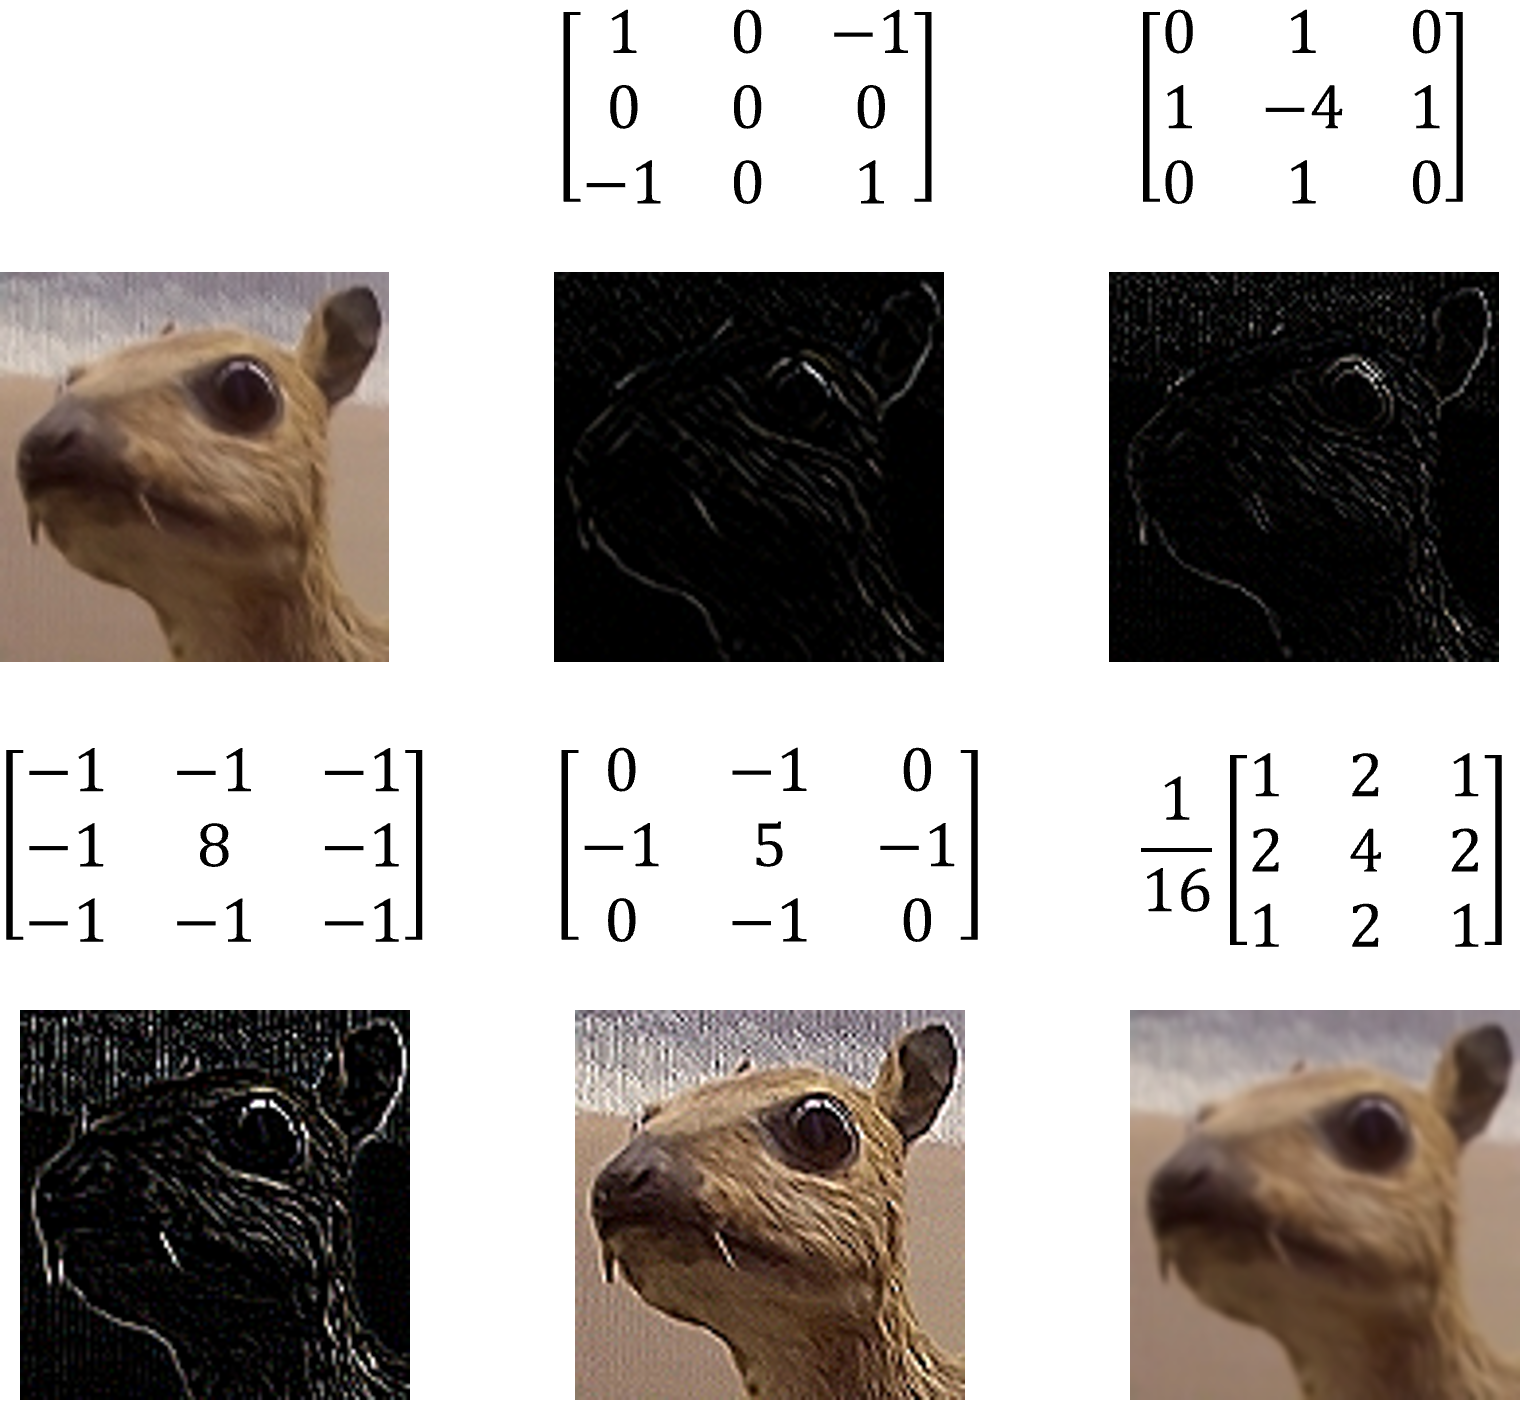
\includegraphics[width=1.0\textwidth,height=0.8\textheight,keepaspectratio]{images/cnn/conv_12.png}
\caption*{\scriptsize [Source: \url{https://medium.com/analytics-vidhya/understanding-convolution-operations-in-cnn-1914045816d4}]}
\end{figure}

\end{frame}
